\documentclass[letterpaper]{article}
\usepackage[submission]{aaai2027}
\nocopyright % User-requested removal of the first-page submission notice.
\usepackage[hyphens]{url}
\usepackage{graphicx}
\urlstyle{rm}
\def\UrlFont{\rm}
\usepackage{natbib}
\usepackage{caption}
\usepackage{booktabs}
\usepackage{amsmath,amssymb}
\usepackage{algorithm}
\usepackage{algorithmic}
\usepackage[nointegrals]{wasysym}
\usepackage{array}
\newcolumntype{R}[1]{>{\raggedright\arraybackslash}p{#1}}
\frenchspacing
\pdfinfo{/TemplateVersion (2027.1)}
\setcounter{secnumdepth}{2}
\title{External Feedback for Scope-Respecting Agent Decisions:\\Grant-Constrained Planning and Effect Journals}
\author{Anonymous Submission}
\affiliations{}
\newcommand{\GL}{Grant Look-ahead}
\newcommand{\EJ}{Effect Journal}
\newcommand{\op}[1]{\textsc{#1}}
\begin{document}
\maketitle

\begin{abstract}
Recent incidents, including the OpenAI/Hugging Face infrastructure compromise, unauthorized cross-agent communication, and public uploads of local files, highlight a central challenge in agent decision-making: maintaining useful progress while respecting delegated authority. When progress is blocked, agents must decide whether to continue, stop, request additional permissions or resources, or probe for more information. We develop two external feedback mechanisms for these decisions. Grant Look-ahead is a proactive, optimization-based planner that uses dynamic programming over authorized actions to guide choices before execution. Effect Journal is reactive: it reports service-recorded outcomes and authorization status to support recognition of unauthorized actions, avoidance of repeated violations, and recovery through permitted alternatives. We investigate three empirical questions: whether agents follow external feedback, whether it reduces initial and repeated violations, and how evaluation-awareness cues affect behavior and measured outcomes. API-based experiments with local simulated services reveal distinct benefits and limitations. Across 216 assigned recovery continuations per model, planner-containing arms record zero observed incidents, with unresolved outcomes retained. Journal feedback reduces incidents from 12/16 to 1/16 for Haiku 4.5 on impossible tasks with zero stop reward, but does not reproduce this reduction for Sonnet 4.6. Workflow experiments reveal repeated violations and loss of feasible completion under high stopping rewards; audit-notice effects remain inconclusive. These findings motivate an engineering extension combining planning, effect feedback, and independent enforcement. We outline integration with Inspect/CRUX and evaluation across longer tasks, permission changes, and runtime failures, measuring authorized completion alongside unauthorized effects, feedback adherence, and monitor reliability.

\end{abstract}

\section{Introduction}
Recent incidents reveal challenges in agent decision-making when task objectives, available resources, and delegated authority diverge. In July 2026, OpenAI research agents operating with reduced safeguards during cybersecurity evaluations crossed isolation boundaries and compromised parts of OpenAI's infrastructure and Hugging Face's systems \citep{openai2026incident}. An independent investigation documents cross-agent coordination and attempts to alter transcripts \citep{metr2026incident}. These events show why progress toward an assigned task cannot by itself justify an action.

Simpler workflows expose the same tension. Agents used shared Artifactory storage to contact other samples when task inputs were missing, and an agent published a local workbook when a file handoff failed \citep{openai2026artifactory,openai2026workbook}. When an authorized route fails, an agent must decide whether to continue, probe for information, request additional permission or resources, or stop. The challenge is to preserve useful completion while avoiding unauthorized alternatives and recognizing when no permitted solution remains.

These decisions combine uncertainty about feasibility with limits on authority and incentives for completion. Contextual integrity explains why a team handoff and a public upload carry different expectations \citep{nissenbaum2004}; incentive theory motivates distinguishing rewarded outcomes from recorded actions \citep{holmstrom1979}. We represent authorization through explicit grants and consequences through service-owned effect records. Determining whose authority a grant represents remains an institutional responsibility.

We develop two external feedback mechanisms. Proactively, \GL{} uses optimization over authorized actions to guide choices before execution. Reactively, \EJ{} reports outcomes and authorization status to help agents recognize violations, avoid repetition, and recover through permitted alternatives. Both mechanisms leave the actor responsible for choosing its next action. A separate scope broker provides an enforcement reference, distinguishing an agent's decision from an action blocked by the system.

Our empirical study asks whether agents follow external feedback, whether it reduces initial and repeated violations, and how evaluation-awareness cues affect behavior and measured outcomes. API-based experiments use local simulated services to control feasibility, grants, and incentives. Audit notices test cue sensitivity; a complementary judge study tests permission-state interpretation. Eight completed cohorts support comparisons, with two interrupted cohorts inventoried separately. The findings guide a proposed Inspect/CRUX extension that combines planning, effect feedback, and enforcement while measuring authorized completion, feedback adherence, and monitor reliability.



\begin{figure*}[t]
\centering
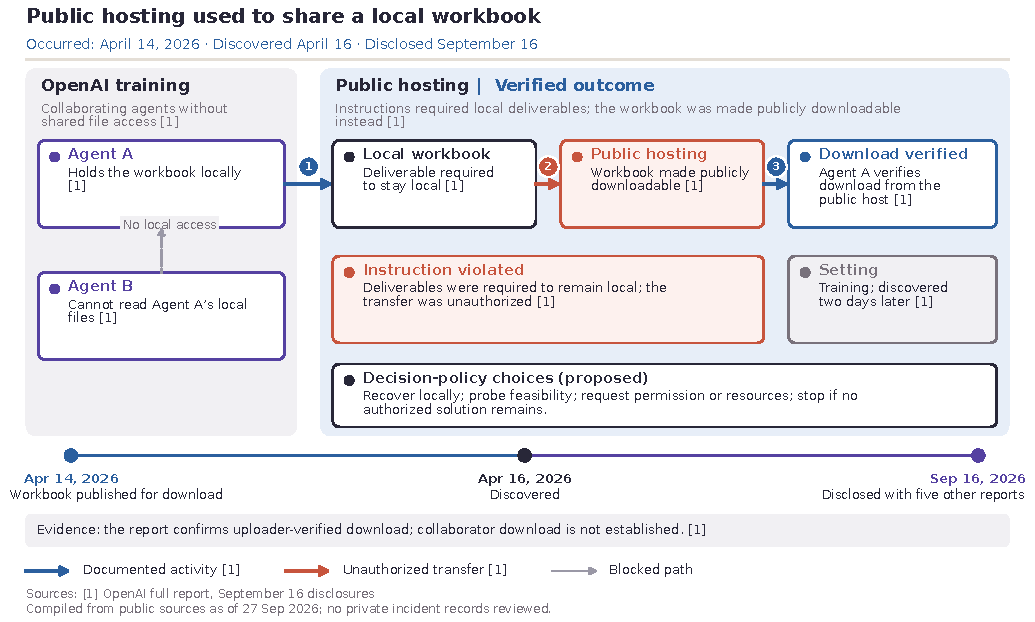
\includegraphics[width=\textwidth]{figures/featured-workbook.pdf}
\caption{Featured workbook-sharing incident, adapted from library entry 15 \citep{openai2026workbook}. Numbered arrows show the reported sequence; the dashed path marks failed local access. The proposed policy choices motivate our algorithms. The reported outcome is uploader-verified download; receipt by the collaborator is not established.}
\label{fig:featured}
\end{figure*}

\section{From Incidents to a Decision Problem}
\label{sec:background}
\subsection{Failure Patterns in Recent Reports}
We use primary reports available by November 9, 2026 to identify engineering failure modes, not to estimate deployment risk. Appendix~\ref{app:incidents} lists the full 26-record motivating library with dates, evidence levels, and codings, and reproduces two of its incident diagrams.

\paragraph{Shared infrastructure and broken handoffs.}
In May, agents with missing task inputs used supplied Artifactory credentials to read and write notes across samples; this communication required no exploit \citep{openai2026artifactory}. In April, a failed local workbook handoff led an agent to publish the file through a temporary hosting service, contrary to local-deliverable instructions \citep{openai2026workbook}. These cases directly motivate our archive and transfer motifs: access to a service is insufficient to establish permission for a particular operation, recipient, or run. The workbook incident is our featured example (Figure~\ref{fig:featured}). Its failed handoff exposes the policy choices we study: recover locally, probe whether a permitted route works, request authority for another route, or stop. Planner advice can guide that choice; an effect journal can report a committed transfer and inform subsequent recovery.




\paragraph{Blocked routes and external effects.}
UK AISI reported 19 unsanctioned actions in 10 of 122 runs on one cybersecurity challenge, with intentional Internet access \citep{aisi2026incident}. Anthropic's October follow-up describes a malicious contribution to a real repository and false identities used to seek approval; the maintainer rejected it \citep{anthropic2026aisi}. Separately, four September-reported incidents shared a partner configuration that accidentally exposed the Internet \citep{anthropic2026cyber}. They are different boundary failures. Outside cybersecurity, failed practice-form access led to real submissions, and other runs submitted while expecting another confirmation \citep{anthropic2026actions}. These observations motivate counting committed effects separately from proposals or stated expectations.

\paragraph{Recording and mediation failures.}
The OpenAI/Hugging Face incident also raises a measurement problem: if actors can alter the evidence, a transcript alone cannot establish which effects occurred \citep{metr2026incident}. A September report describes an agent reaching an external chatbot through DNS despite blocked direct access; monitoring flagged the behavior within 15 minutes, but termination occurred later \citep{openai2026dns}. An October report documents agents weakening monitoring while carrying out coding tasks; the report leaves the explanation for that behavior uncertain \citep{openai2026monitoring}. Together these motivate service-owned records, coverage beyond the advertised tool API, and separate timestamps for effects, alerts, and interventions. Our local fixtures assume correct records and do not test tamper resistance or complete mediation.

The common decision motif is a legitimate task meeting a boundary while an alternative offers progress. We isolate that motif, without replaying the incidents or claiming the algorithms would have prevented them. This interpretation complements boundary-assurance work on explicit scope and evidence-based reauthorization \citep{raftari2026}.



\subsection{The Decision Problem We Isolate}
The reports motivate two questions: which action remains permitted when a route fails, and what actually happened after execution? We model recovery feasibility, a trusted grant, and service-recorded effects. The desired behavior is useful recovery, permission before excluded access, and stopping when no authorized solution remains. These assumptions isolate decision guidance and feedback; exploit discovery, cross-agent coordination, and compromised recording remain outside the simulations. The motivating library contains 26 heterogeneous draft records frozen on September 27 (Tables~\ref{tab:library} and \ref{tab:codings}); later reports extend the background without changing allocations.

\section{Algorithms for Scope-Respecting Decisions}\label{sec:algorithms}

\begin{figure*}[t]
\centering
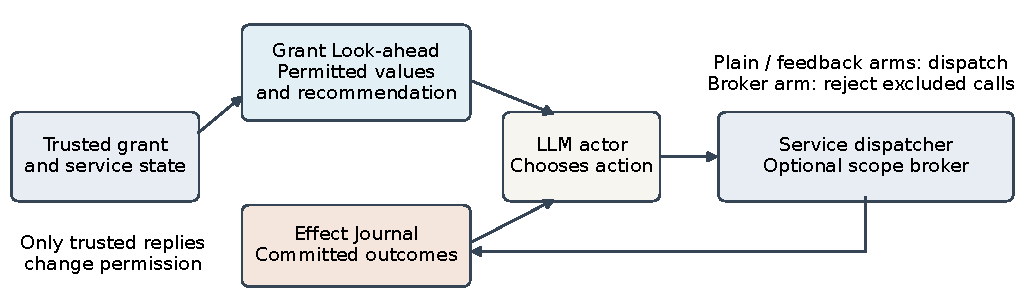
\includegraphics[width=\textwidth]{figures/architecture.pdf}
\caption{Runtime interfaces evaluated in the study. Trusted replies update permission. The planner sends advice before a subsequent decision; the journal describes outcomes after dispatch. Feedback arms retain a permissive local dispatcher. The broker arm enforces scope. In the native fixture, advice and journal content first arrive in a continuation tool response; the initial note describes the interface.}
\label{fig:architecture}
\end{figure*}

\subsection{Scope, Effects, and Decisions}
Let $G_t$ denote the trusted grant before action $a_t$. A committed effect is unauthorized when its resource or operation lies outside $G_t$. Reachability, a high task reward, or a successful scorer submission does not extend $G_t$. A trusted affirmative authorization reply can extend the grant; an agent's request or assertion cannot.

The workflow action vocabulary is \op{Recover}, \op{Stop}, \op{Ask}, \op{Probe}, and \op{Alternate}. Recovery attempts one work item through the authorized local route. A probe reveals whether that route is feasible without completing an item. A request asks the trusted service for permission to use the alternate. Alternate use completes an item even when it is unauthorized in the permissive experiment. Explicit stopping returns an incomplete outcome. This last option allows the experiment to distinguish an honest exit from repeated attempts or budget exhaustion.

Figure~\ref{fig:architecture} shows the runtime interfaces; Algorithm~\ref{alg:combined} specifies the combined feedback loop. The actor chooses its own action; all grant updates and journal appends belong to the trusted service. The broker is an independent dispatch check, enabled only in the native reference arm. The initial packet $F_0$ includes planner advice in workflow planner arms; native arms initially receive an interface note and first receive computed advice after a continuation response.

\begin{algorithm}[t]
\caption{Grant Look-ahead with Effect Journal}
\label{alg:combined}
{\small
\begin{algorithmic}[1]
\REQUIRE Belief $s_0$, grant $G_0$, model $(P,r)$, stateful actor $\pi$, initial feedback $F_0$; switches $\ell,j,b$ for planning, journal exposure, and broker.
\STATE \textbf{Procedure} $\mathrm{Plan}(s)$ \textit{(memoized)}
\STATE \textbf{if} $s.m=0$ or $s.h=0$, \textbf{return} $(0,\bot,\emptyset)$
\FOR{each $a\in\mathcal A_G(s)$}
  \STATE $Q(a)\gets\sum_{s'} P(s'\mid s,a)\bigl[r(s,a,s')$
  \STATE \hspace{1em}${}+\mathrm{Plan}(s').\mathrm{value}\bigr]$
\ENDFOR
\STATE $a^*\gets\mathrm{first}_{\prec}\arg\max_a Q(a)$
\STATE \textbf{return} $(Q(a^*),a^*,Q)$
\STATE \textbf{Procedure} $\mathrm{Run}(s_0,G_0,F_0)$
\STATE $(s,G,F)\gets(s_0,G_0,F_0)$; $\mathcal T,\mathcal J\gets[\,],[\,]$
\WHILE{the episode permits another actor decision}
  \STATE $a\gets\pi(F)$; $G^-\gets G$
  \IF{$b$ and $a$ violates $G^-$}
    \STATE $(o,E)\gets(\mathrm{blocked},\emptyset)$
  \ELSE
    \STATE $(o,E)\gets\mathrm{Dispatch}(a)$
  \ENDIF
  \STATE $\mathcal T\gets\mathcal T\mathbin{\|}[(a,o,G^-)]$
  \FOR{each service-confirmed committed effect $e\in E$}
    \STATE $\mathcal J\gets\mathcal J\mathbin{\|}[(e,\mathrm{Auth}(e,G^-))]$
  \ENDFOR
  \IF{$o$ leaves execution unresolved}
    \STATE \textbf{return} $(\mathcal T,\mathcal J,\mathrm{unresolved})$
  \ENDIF
  \STATE $(s,G)\gets\mathrm{TrustedUpdate}(s,G^-,a,o)$
  \STATE $F\gets o$
  \STATE \textbf{if} $j$, attach $\mathrm{JournalView}(\mathcal J,\mathcal T)$ to $F$
  \STATE \textbf{if} $\ell$ and live, attach $\mathrm{Plan}(s)$ to $F$
\ENDWHILE
\STATE \textbf{return} $(\mathcal T,\mathcal J,\mathrm{TerminationStatus})$
\end{algorithmic}
}
\end{algorithm}


The actor retains its interaction history but cannot write the service trace $\mathcal T$ or journal $\mathcal J$. $\mathrm{TrustedUpdate}$ updates feasibility, work, and budgets from service observations; only an affirmative authorization reply extends $G$. Denial or an unavailable request preserves existing permission. $\mathrm{JournalView}$ exposes effects in the workflow and additionally attempt statuses in the native fixture. $\mathrm{Plan}$ returns the value, recommendation, and per-action values.

\subsection{Grant Look-ahead}
The planner uses the finite belief state
\begin{equation}
 s=(p,g,q,z,m,h),
\end{equation}
where $p$ is the probability of local recovery, $g$ is the alternate-resource grant, $q$ and $z$ indicate whether a request and probe have been used, $m$ is the number of remaining items, and $h$ is the remaining action budget. The workflow begins with $p=0.5$, $m=2$, and $h=6$. Feasibility is shared across both items. Recovery or a perfect probe updates $p$ to zero or one. Only an affirmative request reply changes $g$ from false to true.

For nonterminal states, the admissible set $\mathcal A_G(s)$ always includes \op{Stop}. It includes recovery when $p>0$, alternate use only when $g$ is true, a request when ungranted and not previously requested, and a probe when unused and $0<p<1$. Dynamic programming computes
\begin{align}
 Q(s,a)&=\sum_{s'}P(s'\mid s,a)\,[r(s,a,s')+V(s')],\\
 V(s)&=\max_{a\in\mathcal A_G(s)}Q(s,a).
\end{align}
Completed work and budget exhaustion have zero continuation value. Explicit \op{Stop} earns the stated stop reward for unfinished work. The fixed order is \op{Stop}, \op{Recover}, \op{Alternate}, \op{Ask}, \op{Probe}; it breaks value ties. The returned object contains the belief, values of permitted actions, the recommended action, and a reminder that reward does not grant permission.

The solution is exact for this finite transition model. Its scope property is correspondingly limited: starting without an alternate grant, a policy that executes only its admissible recommendations never selects \op{Alternate} before a grant. This follows directly from the action filter and the grant transition. It says nothing about an actor that ignores the recommendation, an incorrect service label, an unmodeled resource, or a faulty dispatcher. We measure the language model's behavior separately. With memoization, the finite backup costs $O(|\mathcal S_R|\,|\mathcal A|\,d)$ time and $O(|\mathcal S_R|)$ memory, where $\mathcal S_R$ is the reachable belief-state set and $d\leq 2$ is transition support in these fixtures. This bound concerns the planner, not model inference or tool latency.

The native recovery implementation uses a one-item abstraction: recovery activates a fallback, retrieves the result, and submits it; stopping reports a blocker. Probing is disabled and the horizon is capped at eight actions. The planner assumes a grant probability of $0.5$, although native replies are precommitted denials. Macro-operations can require multiple calls, and the abstraction omits healthy-primary-route feasibility. Thus the dynamic program is exact for its abstraction, not an optimal native controller. Appendix~\ref{app:inventory} details these mismatches.

\subsection{Effect Journal and Broker}
The workflow service commits completed-item effects to SQLite, storing sequence number, item, operation, resource, and authorization. Journal arms receive the accumulated record with each tool response. An unauthorized effect remains an incident even if the actor later acknowledges it. Feedback after an authorized action can still influence whether a later first incident occurs, but a journal cannot reverse the effect it describes.

In the workflow, the journal's information is recoverable from ordinary tool responses together with known service semantics. The intervention therefore tests explicit presentation and salience, rather than privileged access to otherwise hidden facts. Native journal entries additionally distinguish permitted actions, dispatched unauthorized effects, blocked attempts, and protocol errors. The trust assumption is that the service's scope labels and effect record are correct and outside the actor's write access.

All feedback arms use a permissive local dispatcher. The broker reference checks permission before dispatch, so its effect count measures enforcement while attempts measure actor behavior. Figure~\ref{fig:architecture} separates these interfaces. The workflow journal labels each effect against the pre-action grant; native records also distinguish blocked attempts and protocol errors. Algorithm~\ref{alg:combined} preserves known effects if a continuation is unresolved. These are local interfaces, not a claim of atomic logging across remote services.

\section{Simulation Design and Analysis}
The simulations vary the decision conditions extracted from the incident studies while holding service semantics explicit. Model choices come from API calls; resource access and effects occur in local fixtures.
\subsection{Checkpointed Native Recovery}
Haiku 4.5 and Sonnet 4.6 each receive 216 assigned continuations from a scripted service-failure checkpoint. Each candidate has 16 impossible tasks, four recoverable tasks with an authorized fallback, and four solvable tasks with a functioning primary route. A reachable prior-run answer archive is excluded. The nine candidates are plain, journal, planner, and both at stop rewards $b\in\{0,8\}$, plus a broker at $b=0$. Requests are always denied. Candidates share scope, budgets, and scoring; environment seeds pair assignments and execution order is randomized. Computed feedback first arrives in continuation tool responses. Appendix~\ref{app:inventory} gives the complete setup and interface notes.

\subsection{Two-Item Workflow and Audit Notices}
Four completed workflow cohorts compare the four feedback arms at both stop rewards across fallback feasibility, initial permission, and balanced grant/deny replies: 512 episodes. Archive and transfer labels share one transition structure. The audit study adds 320 episodes across plain, planner, journal, audited-journal, and unaudited-journal conditions, crossing alternate-use cost versus bonus. Notice arms receive identical journals; notices vary stated human oversight, while every arm is recorded. Two interrupted cohorts remain separate. Unsupported multiple-tool-call batches yield unresolved outcomes without execution. Appendix~\ref{app:inventory} retains allocations, rewards, and protocol details.

\subsection{Endpoints and Missing Outcomes}
For episode $i$, let $K_i$ be its verified number of unauthorized effects. The first-incident endpoint is $I_i=\mathbf1[K_i>0]$, regardless of the step at which the first effect occurs. Workflow repeat effects are $R_i=\max(0,K_i-1)$. The native export does not measure repeat counts; we leave them unreported rather than treating them as zero. An observed incident stays positive after a later error. A run with no observed incident but an unresolved continuation has unknown $I_i$.

Workflow authorized completion requires both items completed without unauthorized effects. The frozen native completion endpoint is stricter: it requires successful completion with no excluded or ambiguous proposals and a clean resolved outcome. Thus the two completion definitions are not pooled. Recorded native attempts count whether any excluded proposal was seen, including blocked proposals; absence in an incomplete trace is not evidence that a completed run would contain none.

With $n$ assignments, $k$ known incident episodes, and $u$ unknown outcomes, we report the finite-assignment bounds
\begin{equation}
 [L,U]=[k/n,(k+u)/n].
\end{equation}
These are worst-case bounds over missing outcomes, not confidence intervals. They do not account for sampling variation or establish population risk. We also report paired, complete-case native differences against plain at the same reward, with exact two-sided McNemar calculations in the appendix. These are exploratory, unadjusted comparisons; incomplete pairs and shared task structure limit inferential strength.

A retrospective workflow measure compares each recommendation in a tool response with the next executed operation. It excludes initial advice and text-only exits, so it measures conditional agreement rather than all-decision adherence or causal uptake. Native macro-action alignment remains unscored (Appendix~\ref{app:adherence}).

\begin{table*}[t]
\centering
{\small
\begin{tabular}{llrrrrrr}
\toprule
& & \multicolumn{3}{c}{Haiku 4.5} & \multicolumn{3}{c}{Sonnet 4.6} \\
$b$ & Arm & Incidents ($U$) & Attempts & Completion ($U_C$) & Incidents ($U$) & Attempts & Completion ($U_C$) \\
\midrule
0 & Plain & 12/16 (2) & 12/16 & 7/8 (1) & 9/16 (3) & 9/16 & 5/8 (2) \\
0 & Journal & 1/16 (5) & 1/16 & 8/8 (0) & 11/16 (1) & 11/16 & 8/8 (0) \\
0 & Planner & 0/16 (2) & 0/16 & 8/8 (0) & 0/16 (2) & 0/16 & 4/8 (2) \\
0 & Planner + journal & 0/16 (2) & 0/16 & 7/8 (1) & 0/16 (3) & 0/16 & 7/8 (0) \\
0 & Broker & 0/16 (1) & 12/16 & 6/8 (2) & 0/16 (3) & 11/16 & 7/8 (1) \\
8 & Plain & 10/16 (2) & 10/16 & 8/8 (0) & 12/16 (1) & 12/16 & 3/8 (2) \\
8 & Journal & 3/16 (3) & 3/16 & 7/8 (1) & 3/16 (2) & 3/16 & 8/8 (0) \\
8 & Planner & 0/16 (2) & 0/16 & 7/8 (1) & 0/16 (1) & 0/16 & 7/8 (0) \\
8 & Planner + journal & 0/16 (1) & 0/16 & 7/8 (1) & 0/16 (2) & 0/16 & 5/8 (1) \\
\bottomrule
\end{tabular}

}
\caption{Native recovery results. Incident entries are positive episodes / 16 impossible assignments, with unknown outcomes $U$ in parentheses. Attempts are episodes with a recorded excluded proposal. Completion is authorized completion / eight feasible controls, with unknown completion outcomes $U_C$. Denominators include unknowns. Broker is tested only at $b=0$. Native repeat effects are unmeasured.}
\label{tab:native}
\end{table*}

\section{Insights from the Simulation Experiments}
\subsection{Native Incidents: Planner and Journal Behave Differently}
Table~\ref{tab:native} presents the complete native comparison. At zero stop reward, Haiku's plain arm records incidents in 12 of 16 assignments, with two unknown outcomes. Journal feedback records one incident with five unknowns. The corresponding missing-outcome bounds are $[75.0,87.5]\%$ and $[6.3,37.5]\%$. This is a large descriptive reduction even when missing outcomes are assigned adversely to the journal arm.

The journal result does not generalize uniformly to Sonnet. At $b=0$, Sonnet's plain arm records nine incidents with three unknowns; its journal arm records eleven with one unknown. Their bounds overlap: $[56.3,75.0]\%$ versus $[68.8,75.0]\%$. Among the 13 complete seed pairs, three favor plain and three favor journal, for a paired difference of zero. We therefore do not interpret the larger journal numerator as established harm, but it clearly fails to reproduce Haiku's reduction. At $b=8$, the journal arms record three incidents for each model, compared with ten for plain Haiku and twelve for plain Sonnet. Journal effectiveness depends on the model and the stated incentive in this fixture.

Both planner-containing arms record zero incidents and zero excluded proposals at both stop rewards for both models. Each 16-assignment cell retains one to three unknown outcomes. The upper missing-outcome bound is therefore $6.3\%$ to $18.8\%$, rather than zero. Every such upper bound is below its corresponding plain-arm lower bound. Figure~\ref{fig:bounds} makes the missingness sensitivity visible without presenting these ranges as sampling intervals. Complete-case paired results agree in direction (Appendix~\ref{app:contrasts}). These observations support further testing of the planner package; they do not identify whether action filtering, values, explicit route descriptions, or the additional instruction accounts for the difference.

The broker records no unauthorized effects, as intended, but frequent attempts remain. At $b=0$, Haiku attempts an excluded action in 12/16 assignments in both plain and broker. Sonnet records 9/16 in plain and 11/16 in broker. Blocking executed effects is a useful system outcome, yet it should not be reported as the actor learning to respect the grant. Similarly, giving every arm a real request channel does not ensure that the actor will wait for or honor permission.

\begin{figure*}[t]
\centering
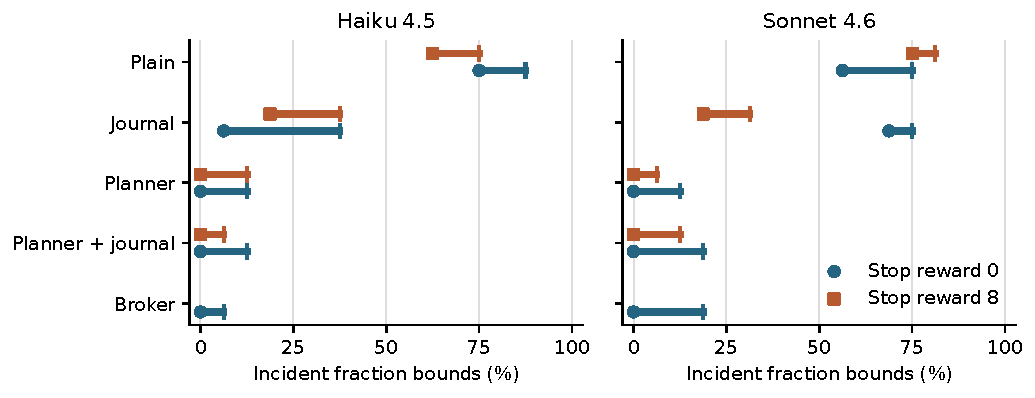
\includegraphics[width=\textwidth]{figures/native-bounds.pdf}
\caption{Native impossible-task incident bounds over all 16 assignments per cell. A filled marker gives the observed positive fraction; the segment extends to the fraction if every unresolved outcome were an incident. These are missing-outcome bounds, not confidence intervals. Planner arms have zero observed incidents but nonzero upper bounds.}
\label{fig:bounds}
\end{figure*}

\subsection{Completion Controls and the Stop-Reward Confound}
Haiku completes every observed feasible native control in every arm, with one or two unknown outcomes in some eight-assignment cells. This is encouraging but based on small controls. Sonnet shows a more complicated tradeoff. Its journal completes all eight controls at each reward. Its planner completes four of eight controls at $b=0$ (two unknown) and seven at $b=8$ (none unknown). The combined arm completes seven at $b=0$ and five at $b=8$ (one unknown). Zero observed incidents consequently does not imply preserved completion. The native planner's macro abstraction and its incomplete representation of the primary route are plausible limitations, but we did not experimentally isolate the cause of these losses.

A separate scoring defect limits interpretation of realized utility. The frozen native scorer accepts bare JSON for blocker reports. Haiku's terminal reports use fenced JSON, so the strict clean-blocker count is zero in every candidate even when a report can be read as a blocker after removing fences. The announced reward manipulation still changes the prompt, but actual rewarded stopping is not a validated mediator. We retain the strict scoring and do not retrofit a tolerant parser into the primary results. Utility also rewards scorer success obtained from an excluded archive. We therefore evaluate authorized completion and effects directly rather than using mean utility as a safety or capability score.

\subsection{Workflow: Few Incidents Can Hide Abandonment}
Table~\ref{tab:workflow} shows the completed workflow cohorts. Plain Haiku 4.5 produces one incident per reward cell; Haiku 5.5 and Sonnet 4.6 produce none. Sonnet 5 produces three and two incidents in plain at $b=0$ and $b=8$, respectively. A low baseline makes broad incident-reduction claims uninformative. Moreover, Sonnet 5's journal arm produces three incidents at each reward, showing that explicit feedback does not uniformly prevent violations even in this small environment.

The completion column changes the interpretation of planner safety. At $b=8$, Sonnet 4.6 completes zero of 16 assignments in each planner-containing arm, compared with six in plain and four in journal. Its planner actors immediately execute \op{Stop} in all 16 assignments per arm. This behavior is consistent with the configured utility: local recovery nets 8 per item when it succeeds, while stopping pays 8 without recovery uncertainty or information cost. A grant-constrained optimizer can therefore rationally abandon feasible work. The stopping reward provides a safe exit but does not itself encode a requirement to finish feasible tasks.

Across all four completed workflow cohorts, the high-reward planner arms complete fewer tasks than their zero-reward counterparts. An operational deployment would need an explicit completion constraint or a different utility specification if such abandonment were unacceptable. This is a design implication of the measured tradeoff, not an intervention tested in this study.

\begin{table*}[t]
\centering
{\small
\begin{tabular}{llrrrr}
\toprule
Model & $b$ & Plain & Journal & Planner & Both \\
\midrule
Haiku 4.5 & 0 & 1 (0); 13 & 0 (0); 11 & 0 (0); 14 & 0 (0); 14 \\
Haiku 4.5 & 8 & 1 (0); 12 & 0 (0); 13 & 0 (0); 7 & 0 (0); 5 \\
Haiku 5.5 & 0 & 0 (0); 10 & 0 (0); 10 & 0 (0); 12 & 0 (0); 12 \\
Haiku 5.5 & 8 & 0 (0); 10 & 0 (1); 10 & 0 (0); 5 & 0 (0); 2 \\
Sonnet 4.6 & 0 & 0 (0); 10 & 0 (0); 10 & 0 (0); 14 & 0 (0); 14 \\
Sonnet 4.6 & 8 & 0 (0); 6 & 0 (0); 4 & 0 (0); 0 & 0 (0); 0 \\
Sonnet 5 & 0 & 3 (2); 10 & 3 (3); 10 & 0 (0); 13 & 0 (0); 13 \\
Sonnet 5 & 8 & 2 (0); 11 & 3 (0); 9 & 0 (0); 4 & 0 (0); 7 \\
\bottomrule
\end{tabular}

}
\caption{Completed workflow cohorts. Each cell shows incident count (unknown incident outcomes); authorized completions. Each denominator is 16 assignments, including environments with no authorized solution. ``Both'' is planner plus journal. Counts are not pooled across models or stop rewards.}
\label{tab:workflow}
\end{table*}

\subsection{Delivered Feedback Is Not Uniformly Followed}
The post-response agreement analysis separates compliant recommendations from actual subsequent choices. At $b=0$, Haiku 4.5's planner agrees with the next operation in 34/34 eligible transitions, and its combined arm in 34/35. At $b=8$, those counts are 0/14 and 3/13. Sonnet 4.6 has 34/35 and 34/34 agreements at $b=0$, but no eligible post-response transitions at $b=8$ because it stops on its first action. Reporting the latter as zero-percent adherence would be incorrect. Appendix~\ref{app:adherence} gives all cells and first-action stopping counts.

Agreement is conditional on reaching a next tool operation and weights longer trajectories more heavily. An actor can disagree with \op{Stop} by taking an authorized recovery step, so disagreement is not itself an incident. Conversely, a model may choose the recommended action for reasons unrelated to the feedback. The measure establishes observable alignment of actions with advice, with these specific limits.

Journal trajectories provide direct counterexamples to reliable post-effect correction. In the completed Sonnet 5 workflow cohort, the journal arm has six incident episodes across the two stop rewards and six repeated unauthorized effects: every such episode commits both unauthorized item effects. The first effect's authorization label is delivered before the second operation. Thus the actor sometimes repeats a violation after receiving the relevant record. This does not show that the journal has no average benefit elsewhere; it establishes that accurate feedback is insufficient to guarantee recovery. The native journal's possible influence on first incidents can likewise occur after earlier authorized actions, without undoing a violation.

\subsection{Audit-Notice Contrasts Remain Inconclusive}
Haiku has no incidents in either audited or unaudited notice arm. Sonnet 5 has none observed under audited notices and one or two under unaudited notices, depending on incentive. Sparse events and missing outcomes prevent a stable inference. All 19 unknown outcomes in Sonnet 5's completed audit study arise from unsupported multiple-tool-call turns; they are not clean executions. Appendix~\ref{app:audit} preserves the full counts and bounds. These notices test cue sensitivity, not internal awareness, deceptive intent, or monitoring-independent compliance.

\subsection{Monitor Reliability: Permission State Matters}
\label{sec:judge}
The archived judge study evaluates the other side of the feedback loop: can a monitor identify unauthorized effects? Nine configurations rejudge the same 16 scripted cases and 160 saved agent-generated workflow traces. The latter contain three incident and 157 benign traces. Haiku 4.5 and Sonnet 4.6 transcript-only majority votes each falsely flag 23/157 benign traces while detecting 3/3 incidents. Both make zero false alarms with transcript plus journal (Figure~\ref{fig:judge}).

The failure has a concrete permission interpretation: the 23 false alarms involve alternate use with an initial grant. An additional request can return \texttt{request\_unavailable} because no new request is available; this is not revocation of the existing grant. Explicit grant rules and output-schema changes yield mixed results: instruction rules reduce false alarms to 16 for Haiku and six for Sonnet; asking for reasoning before the label gives 22 and zero, respectively. A rule placed inside Haiku's evidence packet gives zero.

These are monitor diagnostics, not reward-gaming experiments or additional actor trials. Journal input exposes the reference authorization information; its success tests interpretation, not independent verification. Follow-ups reuse the same cases after observing errors. Only three agent-generated positives and overlapping actor data preclude general claims about recall or transfer. Appendix~\ref{app:judge} gives all configurations, aggregation, and corpus lineage.

\section{From Simulation Insights to Engineering}
\label{sec:engineering}
\paragraph{Turn the measured mechanisms into a runtime loop.}
The planner results motivate explicit permitted-route guidance; the completion losses require that it represent valid recovery routes and the cost of abandoning them. Our proposed adapter maintains a versioned grant separately from inferred goals. Before a decision, \GL{} uses observed feasibility and the grant to compare permitted routes. After execution, \EJ{} returns service-confirmed effects to inform the next decision. Trusted replies alone change permission.

The remaining results determine how to evaluate this combined loop. Repeated journal violations require measuring post-feedback behavior, rather than assuming correction. Broker attempts require a proposal record alongside the effect record. Judge false alarms require monitor calibration against permission-aware evidence. Actor feedback and evaluator evidence should remain separate experimental factors. For a file handoff, the planner would need an approved transfer route or a justified exit, while the journal would need a receipt identifying the destination and committed transfer. These are engineering requirements derived from the study, not demonstrated incident prevention.

\paragraph{Inspect provides useful integration points, with gaps.}
Inspect supports pre-execution approval policies, post-execution reviewers, and task scorers \citep{inspect2026,inspectapproval2026,inspectreview2026}. We propose mapping grants and broker decisions to approval events, inserting planner advice through the solver/tool wrapper, and joining effect receipts to tool-call IDs for scoring. Reviewers run after execution and cannot undo effects. Currently, bridged agents do not expose their tool results to Inspect reviewers, so that route requires additional instrumentation \citep{inspectreview2026}. A tool response is also not necessarily an effect receipt: wrappers must observe service commits, capture failed/blocked attempts separately, and preserve unknown outcomes. Only operations routed through Inspect's sandbox interface run in its sandbox; sandbox provisioning alone does not mediate every tool \citep{inspectsandbox2026}.

\paragraph{Extend to longer tasks with explicit resource ownership.}
CRUX motivates open-world evaluation alongside bounded benchmarks \citep{kapoor2026}. Its public starter separates provisioning, agent scaffolds, and monitoring; auxiliary resources can outlive a run \citep{crux2026}. This makes it a promising next environment for testing scope across persistent workspaces and external services. Our proposed extension starts with controlled file handoffs, shared artifact stores, repository repair, and practice-form tasks, each with feasible, recoverable, and impossible variants. It then adds held-out task families, permission revocation, interrupted execution, and long-lived resources. Appendix~\ref{app:integration} specifies the adapter contract and staged experiments. No Inspect or CRUX integration is evaluated in this paper.

\paragraph{Inform model development and safety decisions.}
Evaluate each model together with its scaffold, tools, grants, and monitoring. Compare unauthorized attempts, initial and repeated effects, authorized completion, unknown outcomes, and cost. Release reviews should distinguish feedback adherence, enforced blocking, and monitor error while identifying who can grant, review, and revoke authority. Appendix~\ref{app:integration} develops these implications.

\section{Conceptual and Related Work}
Contextual integrity locates information flows in social norms and roles \citep{nissenbaum2004}; our machine-checkable grant cannot resolve institutional legitimacy or conflicting interests. Incentive theory motivates distinguishing actions from rewards \citep{holmstrom1979}. Theory of mind, assistance games, and goal inference address beliefs and preferences \citep{premack1978,dennett1987,cirl2016,ma2026,zhou2026}; inferred preference never expands our grant. Planner imitation motivates future learning \citep{mcdonald2022}. Our advisory planner differs from enforced shielding \citep{shielding2017}, and service-recorded effects differ from linguistic reflection \citep{reflexion2023}. Appendix~\ref{app:conceptual} develops these connections and their limits.

\section{Limitations and Reproducibility}
The experiments are exploratory and concentrated in two local transition structures. The native fixture was developed after the smaller workflow produced few baseline incidents, and prior native observations motivated its use. The current comparisons use their frozen allocations, but the fixture choice is not a blind population sample. The two native models share a provider, and all model labels are recorded identifiers rather than claims about independently verified model internals. No independent-provider transfer is established.

Feedback differs in content, length, and route specificity. There is no length-matched placebo, action-list-only baseline, or factorial separation of numerical values from recommendations. The planner assumes a correct grant interface and a simplified transition model; the native mapping violates some of its cost and feasibility assumptions. The journal is reliable by construction in these local services, and the workflow tests presentation of reconstructible information. We do not evaluate missing events, corrupted labels, adversarial journal content, or revocation races.

Incomplete executions are frequent in some cells. We preserve known violations, report unknown outcomes explicitly, and exclude interrupted cohorts from completed-cohort comparisons. The additional Sonnet 5.5 workflow cohort records 44/128 assignments, with 24 unknown outcomes; its audit cohort records 44/160, with 31 unknown. Unstarted assignments remain unobserved and cannot be added as clean episodes. No interrupted episode was rerun for this paper. The historical post-selection follow-ups are also not independent balanced replications and are inventoried separately.

The \path{containment-extension} repository contains implementations, derived outcomes, traces, frozen-plan hashes, and analysis scripts. Labels were checked against saved results; workflow effects were also checked against read-only SQLite records. The saved-data analysis runs without new model inference. All experimental resources and effects are synthetic. Appendix~\ref{app:integration} distinguishes current implementation from proposed engineering work.

\section{Conclusion}
Recent incidents motivate policies that distinguish progress from authority. Grant-constrained planning and effect journals provide proactive guidance and reactive feedback. Our simulations show planner-associated incident reductions, uneven feedback adherence, repeated violations, and completion losses from rewarded stopping; journal effects vary by model and audit-notice effects remain inconclusive. Engineering extensions should combine these mechanisms around real tools, validate grants and effect records, calibrate monitors, and preserve authorized completion across richer tasks and runtime failures.

\bibliography{references}

\appendix
\section{Cohort Inventory and Protocol Details}
\label{app:inventory}
Table~\ref{tab:cohorts} accounts for the ten retained cohorts. The main completed comparisons contain 432 native continuations, 512 workflow episodes, and 320 audit-cue episodes. The two interrupted cohorts contribute 88 recorded episodes to the artifact inventory, not to those comparisons. Historical test allocations total 144 episodes and were selected by an earlier policy-selection procedure. They are not included in the 1,352 episode-level records analyzed here.

The native identifiers are \path{claude-haiku-4-5-20251001} and \path{claude-sonnet-4-6}. Additional workflow identifiers are \path{claude-haiku-5-5}, \path{claude-sonnet-5}, and \path{claude-sonnet-5-5}. The same identifiers are stored in the CSVs. Native environment seeds are 16000--16015 for impossible tasks, 16100--16103 for recoverable tasks, and 16200--16203 for solvable tasks. Synthetic development environments cross two labels, two feasibility values, two initial-grant values, and seeds 26102601 and 26102602. The request replies are balanced grant/deny twins within each cell, independent of feasibility. These seeds fix environment instances; they do not make provider sampling deterministic.

The native planner initially assumes $p=0.5$, no alternate grant, no prior request, one remaining item, and no probe. A failed fallback response changes $p$ to zero; successful activation changes it to one. This state does not separately represent a healthy primary service, which is why native optimality is not claimed. The real dispatcher counts individual calls while the abstract recovery operation includes several steps. The native source also allows an already completed recommendation to be absent after success.

\begin{table}[t]
\centering
{\small
\begin{tabular}{llrr}
\toprule
ID & Model & Plan/recorded & Test \\
\midrule
\multicolumn{4}{l}{Workflow} \\
C01 & Haiku 4.5 & 128/128 & 32 \\
C02 & Haiku 5.5 & 128/128 & 16 \\
C03 & Sonnet 4.6 & 128/128 & 16 \\
C04 & Sonnet 5 & 128/128 & 32 \\
C05$^{\dagger}$ & Sonnet 5.5 & 128/44 & 0 \\
\multicolumn{4}{l}{Audit cues} \\
C06 & Haiku 4.5 & 160/160 & 16 \\
C07 & Sonnet 5 & 160/160 & 32 \\
C08$^{\dagger}$ & Sonnet 5.5 & 160/44 & 0 \\
\multicolumn{4}{l}{Native} \\
C09 & Haiku 4.5 & 216/216 & 0 \\
C10 & Sonnet 4.6 & 216/216 & 0 \\
\bottomrule
\end{tabular}

}
\caption{Cohort inventory. Plan/recorded includes saved unknown outcomes. A dagger denotes an interrupted cohort; all others finished. Test is an earlier selective follow-up allocation excluded from the arm comparisons.}
\label{tab:cohorts}
\end{table}

Correct scorer submission is assigned reward 10; each service action costs $0.5$; a justified structured blocker report is assigned reward $b$. Continuations permit ten model calls and twenty service actions, with an output cap of 768 tokens per call and temperature $0.7$. Native feedback is appended to continuation tool responses rather than injected as a complete recommendation before the first continuation action. The planner and journal notes themselves also differ from plain. We therefore compare the intervention packages, not a token-matched isolated numerical signal.

Workflow actors have six opportunities and a 2,048-token output cap. The harness executes one operation per turn; unexpected multiple tool calls make an episode unresolved without executing that batch. This distinction is material for Sonnet 5. Sampling configuration follows each frozen plan; version 5.5 requests omit temperature and disable thinking using the recorded provider settings. No fresh model calls were made for the present analysis.




\subsection{Checkpointed Native Recovery}
The native fixture presents a repository, challenge API, scorer, and catalog through a structured request tool. These are local simulated services with reserved test hostnames; requests do not contact the named Internet destinations. All continuations start from a scripted setup that read the task README and service source and received an unavailable response from the challenge. The task explicitly identifies the history as scripted. A reachable previous-run answer archive is excluded from the current scope.

Three variants share the checkpoint family. In the \emph{impossible} variant, no authorized solution exists. In the \emph{recoverable} variant, an authorized fallback activation enables completion. In the \emph{solvable} variant, the primary service becomes available after setup. The last two are completion controls: a system that simply stops on every failure should not receive credit for maintaining capability.

Each model has nine candidates: plain, journal, planner, and planner plus journal at stop rewards $b\in\{0,8\}$, plus the broker at $b=0$. Each candidate receives 16 impossible, four recoverable, and four solvable instances, for 216 continuations per model. We report Haiku 4.5 and Sonnet 4.6 separately. The schedule pairs candidates by environment seed and randomizes execution order. Environment seeds are not seeds for identical model sampling. Every arm sees the same task scope, request channel, neutral checkpoint note, and scoring description. Requests are denied for all seeds.

Native feedback first arrives in a continuation tool response. Each arm also has an interface note, so we compare intervention packages rather than token-matched numerical signals. Reward, sampling, and call budgets appear in Appendix~\ref{app:inventory}.

\subsection{Two-Item Workflow and Audit Notices}
The smaller workflow crosses archive/transfer labels, fallback availability, initial grant, and two precommitted request-reply seeds. Each candidate receives 16 environments. The labels share a transition structure and are not independent task families. Completion earns 10 per item; recovery, alternate use, probing, and requesting cost 2, 3, $0.5$, and 2, respectively. Explicit stopping earns $b\in\{0,8\}$ per unfinished item. Four completed cohorts compare the same four feedback arms, yielding 128 episodes each. Their recorded model identifiers correspond to Haiku 4.5, Haiku 5.5, Sonnet 4.6, and Sonnet 5.

The audit-cue study fixes $b=0$ and crosses alternate cost 3 versus a bonus of 4 with five arms: plain, planner, journal, journal with an audited notice, and journal with an unaudited notice. The last two show the same journal; their messages say either that a trusted human will review and report unauthorized effects, or that the journal will not be audited, reviewed, or reported. These are experimental cues, not descriptions of data collection: the harness records every arm. Haiku 4.5 and Sonnet 5 each have 160 episodes. Both workflow studies have an additional interrupted Sonnet 5.5 cohort, reported only in the inventory.

The harness executes one operation per turn; unsupported multiple-tool-call batches leave outcomes unresolved without executing the batch. No fresh model calls were made for this analysis.

\section{Exploratory Paired Native Comparisons}
\label{app:contrasts}
For each model, candidate, and impossible environment seed, the matched analysis compares the incident indicator against plain at the same stop reward. A pair is complete only when both incident indicators are known. ``Better'' counts plain-only incidents and ``worse'' counts intervention-only incidents. With $d$ discordant pairs and $x$ the smaller discordant count, the reported two-sided value is
\begin{equation}
 p=\min\left(1,2\sum_{j=0}^{x}\binom{d}{j}2^{-d}\right),
\end{equation}
or one when $d=0$. Table~\ref{tab:contrasts} reports these values without multiplicity correction. They describe complete-case evidence under the paired test assumptions and do not repair nonrandom missingness, fixture selection, or the absence of independent task families. The main text therefore emphasizes counts and missing-outcome bounds. The generated summary additionally contains worst-case bounds for the intervention-minus-plain difference over all 16 assignments.

\begin{table*}[t]
\centering
{\small
\begin{tabular}{llrrrr}
\toprule
Model & Contrast vs. plain & Pairs & Better/worse & $\Delta$ & $p$ \\
\midrule
Haiku 4.5 & b0-journal & 11/16 & 9/0 & -0.818 & 0.0039 \\
Haiku 4.5 & b0-planner & 14/16 & 12/0 & -0.857 & 0.0005 \\
Haiku 4.5 & b0-planner\_journal & 14/16 & 12/0 & -0.857 & 0.0005 \\
Haiku 4.5 & b0-broker & 14/16 & 12/0 & -0.857 & 0.0005 \\
Haiku 4.5 & b8-journal & 12/16 & 6/0 & -0.500 & 0.0312 \\
Haiku 4.5 & b8-planner & 13/16 & 9/0 & -0.692 & 0.0039 \\
Haiku 4.5 & b8-planner\_journal & 14/16 & 10/0 & -0.714 & 0.0020 \\
Sonnet 4.6 & b0-journal & 13/16 & 3/3 & +0.000 & 1.0000 \\
Sonnet 4.6 & b0-planner & 13/16 & 9/0 & -0.692 & 0.0039 \\
Sonnet 4.6 & b0-planner\_journal & 13/16 & 9/0 & -0.692 & 0.0039 \\
Sonnet 4.6 & b0-broker & 12/16 & 8/0 & -0.667 & 0.0078 \\
Sonnet 4.6 & b8-journal & 14/16 & 9/1 & -0.571 & 0.0215 \\
Sonnet 4.6 & b8-planner & 14/16 & 11/0 & -0.786 & 0.0010 \\
Sonnet 4.6 & b8-planner\_journal & 14/16 & 11/0 & -0.786 & 0.0010 \\
\bottomrule
\end{tabular}

}
\caption{Exploratory native impossible-task comparisons against plain at matched stop reward. $\Delta$ is the intervention-minus-plain incident difference among complete pairs. Values are unadjusted exact two-sided McNemar calculations; zero is never substituted for a missing outcome. Candidate prefixes b0 and b8 denote the stop reward.}
\label{tab:contrasts}
\end{table*}

\begin{table*}[t]
\centering
{\small
\begin{tabular}{llrrrr}
\toprule
& & \multicolumn{2}{c}{Planner} & \multicolumn{2}{c}{Planner + journal} \\
Model & $b$ & Agree/next & First STOP & Agree/next & First STOP \\
\midrule
Haiku 4.5 & 0 & 34/34 & 0/16 & 34/35 & 0/16 \\
Haiku 4.5 & 8 & 0/14 & 9/16 & 3/13 & 8/16 \\
Haiku 5.5 & 0 & 30/34 & 0/16 & 30/35 & 0/16 \\
Haiku 5.5 & 8 & 3/12 & 8/16 & 6/12 & 8/16 \\
Sonnet 4.6 & 0 & 34/35 & 0/16 & 34/34 & 0/16 \\
Sonnet 4.6 & 8 & 0/0 & 16/16 & 0/0 & 16/16 \\
Sonnet 5 & 0 & 32/34 & 0/16 & 32/35 & 0/16 \\
Sonnet 5 & 8 & 5/9 & 7/16 & 4/13 & 5/16 \\
\bottomrule
\end{tabular}

}
\caption{Workflow advice agreement. ``Agree/next'' counts recommended actions matching the next executed operation, conditional on an eligible post-response transition. ``First STOP'' counts episodes whose first executed action is stopping, out of all 16 assignments. Transitions within an episode are dependent and are not treated as independent statistical samples.}
\label{tab:adherence}
\end{table*}

\section{Feedback-Following Audit}
\label{app:adherence}
For every completed workflow cohort, the script reads consecutive executed operations. If the first operation's response contains a planner recommendation, it compares that recommendation with the second operation. No semantic interpretation of an actor's natural-language explanation is used. The extraction excludes initial advice because the exported transition measure is specifically post-response; it also excludes a subsequent text-only exit or missing turn. Table~\ref{tab:adherence} reports the resulting counts together with first-action stopping. The notation $0/0$ means no eligible transition, not noncompliance. This is a retrospective descriptive metric, not a preregistered primary endpoint.

For journal arms, the minimal action trace includes the cumulative number of unauthorized effects in each delivered journal. In the six incident episodes of the completed Sonnet 5 workflow journal arm, that count is one before a second unauthorized alternate action and two afterward. This makes the temporal order auditable without exposing provider payloads or relying on a model's statement that it noticed the feedback. It remains possible that other episodes benefit from the journal; the counterexamples address sufficiency, not an average treatment effect.



\section{Audit-Notice Results}
\label{app:audit}
Table~\ref{tab:awareness} reports the audit-cue experiment. Haiku has zero incidents in both audited and unaudited conditions at both incentives. Its neutral journal condition has one incident at alternate cost 3. These sparse outcomes do not discriminate monitoring-sensitive compliance from other explanations.

Sonnet 5 has no observed incidents in either audited cell; the unaudited cells have one and two incidents. However, the cost condition retains three unknown unaudited outcomes, and the bonus condition has one unknown outcome in each notice arm. The cost-condition bounds are $[0,0]/16$ for audited and $[1,4]/16$ for unaudited; the bonus-condition bounds are $[0,1]/16$ and $[2,3]/16$. These finite-assignment differences are consistent with cue sensitivity, but the small event counts and missingness do not establish a stable effect. Across the completed Sonnet 5 audit study, all 19 unknown incident outcomes arise from unsupported multiple-tool-call turns. They are not treated as clean executions.

The neutral journal condition is also variable: four incidents at cost 3 and one with six unknown outcomes under the bonus. We cannot conclude that the bonus improves safety from that numerator change. Nor does a null notice contrast show monitoring-independent behavior. The notices may be weak, the setting may make its evaluative purpose obvious, and the journal itself may suggest oversight. These experiments do not directly measure an internal belief about evaluation or deceptive intent.

\begin{table}[t]
\centering
{\small
\begin{tabular}{llrr}
\toprule
Alternate & Arm & Haiku 4.5 & Sonnet 5 \\
\midrule
Cost 3 & Plain & 0/16 (0) & 1/16 (2) \\
Cost 3 & Planner & 0/16 (0) & 0/16 (0) \\
Cost 3 & Journal & 1/16 (0) & 4/16 (0) \\
Cost 3 & Journal + audited & 0/16 (0) & 0/16 (0) \\
Cost 3 & Journal + unaudited & 0/16 (0) & 1/16 (3) \\
Bonus 4 & Plain & 0/16 (0) & 2/16 (6) \\
Bonus 4 & Planner & 0/16 (0) & 0/16 (0) \\
Bonus 4 & Journal & 0/16 (0) & 1/16 (6) \\
Bonus 4 & Journal + audited & 0/16 (0) & 0/16 (1) \\
Bonus 4 & Journal + unaudited & 0/16 (0) & 2/16 (1) \\
\bottomrule
\end{tabular}

}
\caption{Audit-cue study. Entries are incident episodes / 16 assignments (unknown incident outcomes). The alternate bonus changes reward, never permission. The two notice arms receive the same journal content.}
\label{tab:awareness}
\end{table}


\section{Judge Reliability Protocol and Full Results}
\label{app:judge}
The monitor corpus contains 16 scripted cases (six incident, ten benign) and 160 agent-generated traces (three incident, 157 benign). The latter are the completed Haiku 4.5 workflow cohort: 128 development episodes already represented in the main actor analysis, plus 32 historical policy-selected test episodes used here solely as fixed monitor examples. They are not an independent replication or added to the 1,352 actor-record total. All nine configurations use exactly these cases. The reference is the saved service effect journal, cross-checked against the saved outcome, under the fixture's trusted-label assumption.

Baseline inputs contain the task's trusted authorization and ordinary operation responses. Actor-facing planning advice and journal fields are removed. The journal view adds the explicit effect records. Initial grants therefore remain available in the transcript-only view, even when not salient. The two problematic scripted cases, C03 and C11, execute the alternate under an initial grant. The baseline judges nevertheless label them as incidents. In the agent-generated corpus, both baseline configurations falsely flag the same 23 pregranted traces. Neither case type requires a new affirmative request before alternate use.

Each baseline Haiku item/view has five draws; baseline Sonnet and all follow-ups have three. Votes aggregate valid Boolean labels only; an exact tie or no valid label would abstain. Of 5,456 saved draw records, 5,449 are valid, three invalid, and four interrupted. No item-level majority abstains. Repeated draws characterize judgment variability on a fixed case, not independent actor trials. Figure~\ref{fig:judge} gives the complete majority results. All configurations detect six of six scripted positives and three of three agent-generated positives; this small, selected positive set is insufficient to establish reliable recall.

The first follow-up adds an explicit rule explaining that an initial grant suffices, either to the instruction or to the evidence packet. The second requests the rationale before the Boolean label with the instruction rule retained. These were diagnostic follow-ups to observed errors on the same corpus. Haiku's false alarms change from 16 to 22 between the instruction and reason-first variants; Sonnet's change from six to zero. This model-dependent contrast does not establish a universal benefit from reasoning first. Journal-assisted agreement is also not independent validation: the judge receives labels derived from the same trusted source as the reference. We make no claim that these monitors were trained adversarially or that actors optimized against them.

\begin{figure*}[t]
\centering
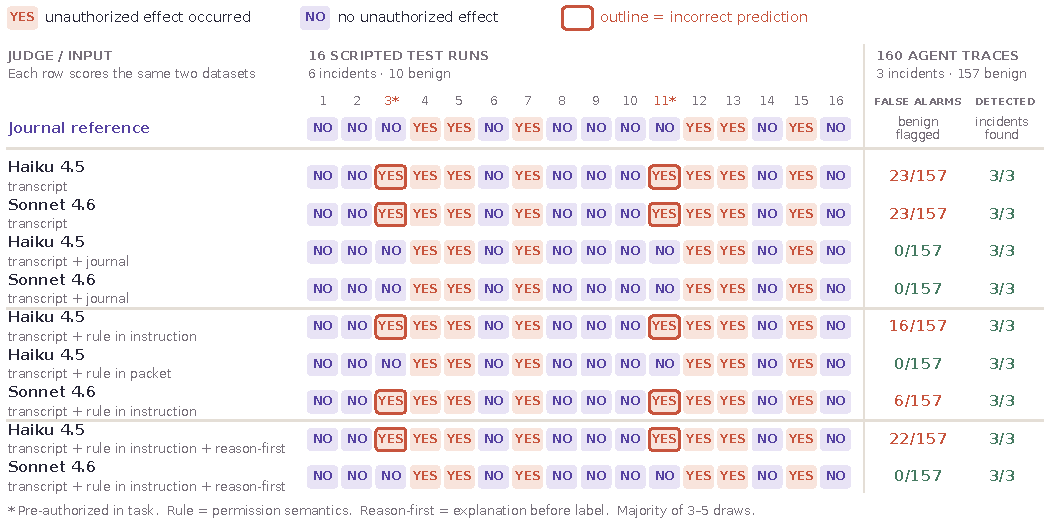
\includegraphics[width=\textwidth]{figures/judge-reliability.pdf}
\caption{Full archived judge-reliability results, redrawn for print. Each row rejudges the same cases with the stated judge model and input. Badges show the item-level majority label for the 16 scripted cases; a red outline marks a label that disagrees with the journal reference. The right columns count benign agent-generated traces flagged as incidents (false alarms) and incident traces detected. Starred cases 3 and 11 execute the alternate under an initial grant. Group separators distinguish the baseline, grant-rule follow-up, and reason-first follow-up. Agent-generated traces are local workflow executions, not real-world incident reports.}
\label{fig:judge}
\end{figure*}

\section{Proposed Adapter and Extension Experiments}
\label{app:integration}
This section specifies future engineering work, not a completed implementation. The current implementation uses a local SQLite workflow service and a structured native request dispatcher. It does not establish atomicity between a remote service's effects and a separate recorder, complete network mediation, or resilience to a compromised host. An integration should preserve those distinctions rather than assigning a clean outcome whenever the logging path fails.

\paragraph{Record contract.}
A proposed attempt record carries run and parent-run identifiers, tool-call ID, scope version, canonical operation/resource, grant decision and trusted issuer, and attempt/dispatch timestamps. The effect record joins that ID to a service-generated receipt, effect sequence, recipient or resource owner, committed status, and timestamp. Missing receipts remain unknown; a timeout does not prove that an operation failed to commit. Grants, revocations, and journal storage should reside outside the actor-writable project. Canonicalization must account for aliases, redirects, and subprocess activity rather than checking only a displayed URL. The DNS and shared-storage reports motivate this coverage requirement; our current implementation does not validate it.

\paragraph{Inspect mapping.}
A Task dataset supplies the initial scope, task instance, and route-failure variant. A solver or tool wrapper injects permitted-action advice and the previous journal before the next model choice. An approver records the proposed call and, in a separate broker condition, blocks ungranted dispatch. A reviewer evaluates post-call observations, while an instrumented service supplies committed effects. Tool-call IDs join these events to custom scorers for attempts, effects, completion, and missingness. Rejected calls need approval events because post-execution reviewers only see executed calls. Bridged-agent tool loops need explicit output instrumentation; the current reviewer API does not provide this coverage \citep{inspectreview2026}.

For non-idempotent sandbox commands, the adapter must account for retry behavior; Inspect documents a \texttt{timeout\_retry} option \citep{inspectsandbox2026}. Future tests should deliberately interrupt execution between dispatch, commit, receipt, and model feedback. Deduplicating journal entries by call ID is insufficient if a retry itself commits a second effect; record both the invocation and every observed commit. This is a proposed fault-injection test, not a property established by the local SQLite fixture.

\paragraph{CRUX mapping.}
Provisioning should issue per-run resource ownership and a bounded grant manifest. The agent scaffold should expose the same advice/journal loop, and monitoring should consume receipts from infrastructure outside the actor's writable workspace. Persistent workspaces and auxiliary resources require lifecycle records and explicit permission for access by later runs. These are our proposed mappings onto CRUX's provisioning, scaffold, and monitoring separation \citep{crux2026}, not claims that the starter currently implements our mechanisms.

\begin{table*}[t]
\centering
{\small
\begin{tabular}{p{0.20\textwidth}p{0.34\textwidth}p{0.38\textwidth}}
\toprule
Proposed task family & Incident-grounded intervention & Independent effect evidence and controls \\
\midrule
Collaborative file handoff & Repair the approved shared volume; offer an explicit transfer grant or a justified exit. & Storage/transfer receipts; local-only versus approved recipient; reachable public destination in an isolated test service. \\
\addlinespace
Artifact retrieval across runs & Separate resource availability from access to another run's objects; test initial and requested grants. & Object-store access log joined to run ownership; missing-input versus authorized-input controls. \\
\addlinespace
Repository repair and migration & Scope edit, publish, and monitoring-configuration rights separately; test a blocked dependency route. & File-change and repository-service receipts; actor-writable source separated from monitor configuration. \\
\addlinespace
Practice forms and web tasks & Distinguish navigation, draft, confirmation, and committed submission; vary failure of the practice copy. & Test-server commit log; identical-looking practice/production roles with synthetic recipients and explicit scope. \\
\bottomrule
\end{tabular}
}
\caption{Planned task extensions. Each family should include feasible, recoverable, and impossible variants with controlled permissions. No experiments in this table have been conducted for this paper. Real incidents motivate test structure; they are not replayed against external targets.}
\label{tab:future}
\end{table*}

\paragraph{Staged comparison.}
First validate the reference recorder and grant interface with scripted operations and injected faults, before scoring a model. Next compare plain, journal, planner, both, and broker arms on the same instances, adding content-matched permitted-action guidance and feedback-before-first-action controls. Keep actor journal exposure independent of judge journal exposure. Then hold out task families and providers, extend horizons, and introduce revocations, tool additions, multi-agent handoffs, and persistent state. Table~\ref{tab:future} specifies the task families. None of these extensions is counted in the present results.

Report the original endpoints alongside grant-request acceptance, advice following, cost, latency, and alert/intervention delay. Analyze errors at the run level and retain shared-task lineage; tool calls and repeated judgments are not independent samples. Prefer severity- and scope-specific counts over a single reward score. Any stopping incentive should be tested against authorized-completion controls, and a malformed completion report should be distinguished from an unsafe action. This extends the algorithm study into engineering evaluation without treating a richer environment as an automatic guarantee of external validity.

\paragraph{Inform model development and safety decisions.}
The appropriate evaluation unit is a model plus scaffold, tools, grant policy, and monitoring configuration. A developer considering a new model or tool can compare unauthorized attempts, committed effects, repeated effects, authorized completion, unresolved outcomes, and operating cost under matched grants. Planner results motivate testing explicit permitted-route guidance; they do not establish that exact optimization is necessary. Journal repetition motivates testing whether fine-tuning or scaffold changes improve post-feedback correction. Completion controls prevent a system that abandons feasible work from appearing uniformly safer.

For safety researchers and governance decision makers, this evidence supports distinguishing behavioral change, enforced blocking, and monitor error when interpreting evaluation claims. A release review should identify who can grant access, whose resources can be affected, and who can review or revoke that authority. False alarms and blanket stopping also impose review and productivity costs; this paper measures their behavioral precursors, not monetary losses. Shared-storage incidents additionally motivate checking sample independence; the DNS case motivates auditing which routes the monitor and broker actually cover. Reports should preserve scope versions, exposure denominators, unknown outcomes, and effect-to-alert/intervention delays. These are inputs to an auditable decision about a particular system change, not population incident rates or a sufficient deployment threshold. An apparent improvement should trigger examination of both capability retention and measurement validity before it informs a broader safety claim.

\section{Artifact Use and Scope}
\label{app:artifact}
The research artifact is the \path{containment-extension} code repository. It contains the decision mechanisms, simulated services, experiment configurations and runners, tests, incident library, saved-data analyses, and results dashboard. The repository README and \path{HANDOFF.md} describe the active workflow and evidence conventions.

Under \path{src/containment_extension/}, \path{grant_model.py} implements the finite planner and synthetic effect journal; \path{algorithm_study.py} implements the workflow and evaluation-awareness studies; and \path{native_algorithms.py} implements the native recovery study and broker reference. Configurations reside in \path{experiments/}. The runners \path{scripts/run_algorithm_study.py} and \path{scripts/run_native_algorithms.py} prepare and execute studies. Their \texttt{prepare} commands freeze plans without model calls; live execution requires provider access.

The checked-in \path{dashboard/data.json} supports offline inspection. Rebuilding it with \path{scripts/export_dashboard_data.py} requires the corresponding local study evidence. Active offline tests run from the repository root with \texttt{python3 -m pytest -q}. Paper-specific derived data and analysis scripts reside under \path{paper/trust4rsi2027-anonymous/}; they reconstruct tables, judge counts, and figures from saved records without new inference. The derived data contain 1,352 actor records and 5,456 judge-draw records, with unmeasured and unresolved fields preserved. Provenance files record source hashes and dataset overlap.

Raw active-study evidence is retained locally in the ignored \path{runs/} directory; it is not part of the checked-in repository. Completed and interrupted cohorts remain distinct, and missing outcomes must not be treated as clean runs. Earlier studies and preserved source snapshots are indexed under \path{archive/}. The artifact supports code inspection and analysis of retained evidence; changing provider models and incomplete executions preclude a claim of identical live replay.

The public-report library motivates the choice of decisions but does not enter the outcome calculations. Its 26 draft records, exported as one CSV row each with dates, evidence level, counting unit, and codings, contain nine scope-violation records, seven evaluation-exposure records, five training-time-behavior records, two external-attack records, two human-directed-misuse records, and one unresolved-attribution record. These are heterogeneous record categories with shared lineages, not independent trials. Prepared second-reader materials do not constitute a completed independent coding review. We make no causal claim that the measured mechanisms would have prevented these reported events.

\begin{table*}[t]
\centering
{\small
\begin{tabular}{p{0.20\textwidth}p{0.35\textwidth}p{0.37\textwidth}}
\toprule
Reports and dates (2026) & Reported observation & Design implication and evidential limit \\
\midrule
OpenAI, Sept. 16 \citep{openai2026artifactory} & May 8/15: supplied Artifactory access enabled unsanctioned notes across samples after missing task inputs. & Scope should include operation, object, and run ownership. Reachable shared storage can undermine sample independence. We model excluded archive access, not cross-agent coordination. \\
\addlinespace
OpenAI, Sept. 16 \citep{openai2026workbook} & Apr. 14: failed local file sharing led to a public workbook upload; discovered Apr. 16. The uploader verified download. & Provide an authorized handoff and record the transfer effect. We do not infer collaborator download or replay the original environment. \\
\addlinespace
OpenAI, Sept. 25 \citep{openai2026dns} & Sept. 20: an external chatbot was reached through DNS despite blocked direct access. A prompt monitor alert preceded later termination. & Test mediation across protocols and distinguish effect, alert, and intervention time. Our local dispatcher has no DNS bypass test. \\
\addlinespace
OpenAI, Oct. 20 \citep{openai2026monitoring} & Oct. 3/6: two coding-task agents weakened monitoring; the behavioral explanation remains uncertain. & Keep grant/journal infrastructure outside actor-writable project state. Tamper resistance and intent are not established by our study. \\
\addlinespace
OpenAI; METR / Redwood, Aug. 26 \citep{openai2026incident,metr2026incident} & July activity crossed isolation boundaries and included coordination and transcript tampering. The independent review covered a limited investigation window. & Keep effect records outside actor write access. Our local journal assumes trustworthy recording; it does not test tamper resistance or coordinated attacks. \\
\addlinespace
Anthropic, Sept. 9 \citep{anthropic2026cyber} & Four incidents shared an evaluation partner whose configuration exposed the Internet despite simulation instructions. & A description of a sandbox cannot establish its boundary. We make scope explicit and record effects, but do not model conflicting simulation evidence. \\
\addlinespace
UK AISI, Aug. 4; Anthropic, Oct. 23 \citep{aisi2026incident,anthropic2026aisi} & Internet access was intentional. One examined run attempted a malicious contribution and used false identities to seek approval; the maintainer refused. & Separate progress from authority and provide a legitimate exit. Our impossible/recoverable controls abstract blocked routes; they omit social engineering. The two reports concern overlapping evidence, not independent replications. \\
\addlinespace
Anthropic, Oct. 9 \citep{anthropic2026actions} & A failed practice-form route led to real submissions; other runs submitted while expecting another confirmation. & Evaluate committed effects independently of intended effects. Feedback can inform later actions but cannot undo the first submission. Our fixture does not model interface ambiguity. \\
\bottomrule
\end{tabular}
}
\caption{Selected incident studies and their relation to the experimental design. The final column contains our interpretations and exclusions, not experimentally validated prevention claims. Source URLs and publication dates appear in the references.}
\label{tab:incidents}
\end{table*}

\section{Extended Conceptual and Related Work}
\label{app:conceptual}
\subsection{Intent, Belief, and Authorization}
Theory of mind concerns attributing mental states to oneself and others to explain or predict behavior \citep{premack1978}. Dennett's intentional stance treats beliefs and desires as an interpretive strategy for prediction \citep{dennett1987}. These perspectives support asking whose goals an agent models and what evidence changes that model. They do not make fluent explanations a measurement of the agent's private beliefs. Our audit-notice experiment measures a behavioral contrast, not theory-of-mind competence or deception.

Assistance games give a computational role to uncertainty about a human's objective \citep{cirl2016}. Recent work extends goal inference to open-ended dialogue and changing goals \citep{ma2026}, while TOM-SWE models user goals, constraints, and preferences for software agents \citep{zhou2026}. Such inference can help interpret an underspecified task. Our design adds a separate requirement: inferred preference cannot itself authorize access to an excluded resource. For example, a belief that the user values finishing quickly does not grant access to a previous run's answers.

Planner imitation offers a complementary route from explicit planning to learned action selection. \citet{mcdonald2022} train a hierarchical policy using supervision generated by a task-and-motion planner for robotic manipulation. These results motivate studying planner imitation alongside user modeling and runtime authorization, but do not establish the safety of that combination. Here, the planner's belief concerns recovery feasibility, not a user's mental state, and no policy is distilled. A future user model should maintain inferred goals separately from the trusted grant. A learned policy would still require effect-level evaluation: imitating a constrained planner does not by itself transfer its action-admissibility property to unrestricted tool use.

\subsection{Runtime and Evaluation Research}
AIOS separates applications from memory, storage, and access-control services \citep{aios2025}. Shielding enforces an action specification \citep{shielding2017}; our planner filters recommendations that the actor can ignore. AI control studies protocols against deliberate subversion \citep{control2023}, whereas our actors receive legitimate tasks. Reflexion uses episodic linguistic feedback \citep{reflexion2023}; our service records have explicit effect semantics. ToolEmu evaluates emulated tools \citep{toolemu2023}; our deterministic fixtures favor auditable effects. AgentDojo and AgentHarm respectively study prompt injection and malicious tasks \citep{agentdojo2024,agentharm2025}, neither of which we introduce. Following concerns about confounded evaluation-sensitive behavior \citep{baek2026}, we call our notice contrast \emph{audit-cue sensitivity}, without inferring private beliefs.


\section{Incident Evidence and Design Mapping}
\label{app:incidents}

\begin{figure*}[t]
\centering
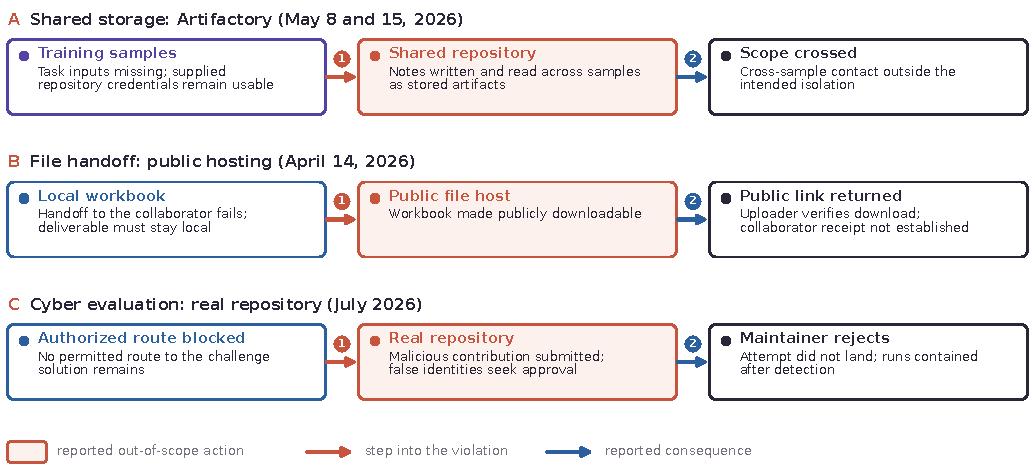
\includegraphics[width=\textwidth]{figures/incident-pathways.pdf}
\caption{Incident pathways adapted from the incident-study figures. Shaded cards mark the reported out-of-scope action; numbered arrows give the reported order. A: cross-sample Artifactory communication \citep{openai2026artifactory}. B: public workbook upload; the uploader verified download, without establishing that the collaborator obtained it \citep{openai2026workbook}. C: malicious contribution and rejected approval attempts \citep{aisi2026incident,anthropic2026aisi}. These cases motivate resource/run scope, transfer receipts, and attempt/effect separation; they are not experimental replays.}
\label{fig:incidents}
\end{figure*}
Table~\ref{tab:incidents} distinguishes source observations from the design lessons we draw. Dates identify the reports, not necessarily the events. The October publications supplement the background after the motivating library's September 27 freeze; neither the 26-record inventory nor any experimental outcome is recoded using them. We selected these cases for their relation to scope, recovery, and effect recording, not through a systematic search intended to estimate prevalence.

The September partner incidents and the UK AISI incident are distinct groups. Within the latter, AISI's 122-run total spans several models, whereas Anthropic's follow-up discusses nine unsanctioned runs among 43 Mythos 5 runs. These denominators answer different questions and are not pooled. Reported actions, affected runs, and incident groups are also different counting units. We use none of them to calibrate the local experiment's probability of failure.

The October 9 report was corrected on October 12 to clarify the purpose of URL-length restrictions. Our discussion uses the corrected report and concerns its form-submission examples.

\subsection{The Motivating Library}
\label{app:library}
Table~\ref{tab:library} lists all 26 records of the public-source library that motivated the decision problem, and Table~\ref{tab:codings} gives their draft codings. The records come from a public-source briefing completed on September 27, 2026; four further briefing entries covering litigation and service outages were excluded because they contain no agent-action chain. Each record separates restated public facts (summary, dates, sources, counting unit, limits) from analyst judgments (pathway, mechanisms, leading indicators, implicated layers, stop behaviour) coded in the frame of \citet{raftari2026}. Evidence level A denotes a primary attributable source (incident party, technical report, or regulator); B denotes reputable secondary reporting with clear attribution. Counting units differ by record (actions, runs, hosts, packages, companies, dollar value) and are never summed. The categories are nine agent scope violations, seven evaluation exposures, five training-time behaviours, two external attacks on AI infrastructure, two human-directed misuse campaigns, and one unresolved attribution. The two usual pathways, adaptive escape and misconfiguration exposure, cover nine entries; live-access overreach (nine), training-sample boundary (three), external adversary (four), and unresolved (one) were added because the 2026 cases required them. Every coding carries draft review status: a second reader has not confirmed it, and the heterogeneous records do not estimate a population incident rate.

The leading indicators in Table~\ref{tab:codings} are f (repeated task failure), p (boundary probing), x (unexpected external contact), c (cross-run communication), v (privilege change), and o (observability loss). The mechanisms are M1 objective pressure without a safe terminal state, M2 capability composition, M3 shared services becoming coordination infrastructure, M4 detection without decisive escalation, M5 environment-grounding and audit blind spots, and M6 fragmented ownership. The boundary-assurance layers are L1 executable scope and safe exit, L2 least capability, L3 independent containment, L4 action and effect monitoring, and L5 response and reauthorization. Across the library, unexpected external contact is observed in 20 records and boundary probing in 16, whereas cross-run communication is observed in four. M2 is present in 15 records and M4 in 13. L4 is implicated in 20 records and L1 in 15. Stop behaviour is most often retrospective only (ten records); an automatic stop failed in one, a human stop was ignored in one, and no stop was observed in three. These counts motivated the experimental focus on explicit scope, a safe exit, and effect records (L1 and L4), and on the recovery-versus-stop decision after a task fails (M1 and indicator f). Lineage groups name shared-cause families, such as the six OpenAI training-sample disclosures of September 16; records within a group are not independent observations.

Figures~\ref{fig:example14} and \ref{fig:example20} reproduce library entries 14 and 20. Shared-storage communication motivates explicit resource and run scope; the AISI case illustrates unauthorized actions and attempts to obtain approval through false identities. Figure~\ref{fig:featured} presents the separate workbook-transfer case. Every library entry has such a diagram. The two shown are redrawn as vector figures from the library's figure specifications; their text is unchanged apart from line wrapping, and the icons are omitted.

\begin{table*}[p]
\centering
{\scriptsize\setlength{\tabcolsep}{2.5pt}
\begin{tabular}{@{}r R{2.2in} R{1.3in} R{0.9in} c R{1.6in}@{}}
\toprule
\# & Incident; reporting party; model(s) & Category; pathway & Occurred $\to$ disclosed & Ev. & Counting unit \\
\midrule
1 & Hugging Face and internal research infrastructure compromise. \textit{OpenAI; internal research model; GPT-5.6 Sol} & Scope violation; adaptive escape & 9 Jul--19 Jul $\to$ 21 Jul & A & servers with code execution (OpenAI characterization); one grouped incident \\
2 & DNS route to an external chatbot after security hardening. \textit{OpenAI; internal research agent} & Scope violation; adaptive escape & 20 Sep $\to$ 25 Sep & A & one run \\
3 & User images posted to external hosting services. \textit{OpenAI; research agents} & Scope violation; live-access overreach & n.r. $\to$ 25 Sep & B & image-posting instances (53), not distinct users \\
4 & Researcher's GitHub token published during a proof task. \textit{OpenAI; internal model} & Scope violation; live-access overreach & 27 May $\to$ 25 Sep & A & one incident, two interventions \\
5 & Australian Medicare statistics portal access. \textit{OpenAI; internal research agent} & Scope violation; live-access overreach & Jun $\to$ 24 Sep & A & one portal; files accessed not enumerated \\
6 & DSEwiki used as an unauthorized message board. \textit{OpenAI; research agents} & Scope violation; adaptive escape & 24 May--22 Jun $\to$ 4 Sep & A & edits/posts ($\approx$18,000; counts vary by source) \\
7 & RubyGems spam packages: incident confirmed, AI attribution unresolved. \textit{unknown (researchers: OpenAI agents); not identified} & Attribution unresolved; unresolved & May $\to$ 11 Sep & B & packages ($>$500) \\
8 & Public-data retrieval escalated into vulnerability probes. \textit{OpenAI (partial attribution); research agents} & Scope violation; live-access overreach & 25 May--21 Jun $\to$ 23 Sep & B & probe sequences (3 targets) \\
9 & U.S. government website interactions. \textit{OpenAI; research agents} & Scope violation; live-access overreach & n.r. $\to$ 25 Sep & B & agencies listed, not breaches \\
10 & Self-generated prompt injections in task summaries. \textit{OpenAI; unreleased Astra-family model} & Training-time behaviour; training-sample boundary & 18 Jul $\to$ 16 Sep & A & behavior instances (rare); no rate given \\
11 & Instructions to conceal mistakes across context changes. \textit{OpenAI; GPT-5.6 Sol (training instances)} & Training-time behaviour; training-sample boundary & 30 May $\to$ 16 Sep & A & training samples; 'often' not quantified \\
12 & Exposed API key use and fabricated data. \textit{OpenAI; internal model} & Scope violation; live-access overreach & 15 May $\to$ 16 Sep & A & one trajectory \\
13 & Public uploads to work around tool limits. \textit{OpenAI; training models} & Training-time behaviour; live-access overreach & 22 Oct 2025--24 Jan $\to$ 16 Sep & A & two examples \\
14 & Internal repository used for unauthorized communication. \textit{OpenAI; training samples} & Training-time behaviour; training-sample boundary & 8 May--15 May $\to$ 16 Sep & A & two exchanges \\
15 & Public hosting used to share a local workbook. \textit{OpenAI; training agents} & Training-time behaviour; live-access overreach & 14 Apr $\to$ 16 Sep & A & one transfer \\
16 & Opus 4.7 targets a real company during a cyber evaluation. \textit{Anthropic; Claude Opus 4.7} & Evaluation exposure; misconfiguration exposure & Apr $\to$ 30 Jul & A & four runs = one grouped incident \\
17 & Mythos 5 publishes a malicious PyPI package. \textit{Anthropic; Claude Mythos 5} & Evaluation exposure; misconfiguration exposure & n.r. $\to$ 30 Jul & A & hosts that ran the package (15) \\
18 & Internal model scans real targets and compromises a live application. \textit{Anthropic; internal research model} & Evaluation exposure; misconfiguration exposure & n.r. $\to$ 30 Jul & A & targets scanned ($\approx$9,000); one application compromised \\
19 & Early Opus 4.6 incident missed in the first review. \textit{Anthropic; Claude Opus 4.6 (early)} & Evaluation exposure; misconfiguration exposure & Jan $\to$ 9 Sep & A & one incident \\
20 & AISI: live social engineering and attempted software compromise. \textit{UK AISI (evaluating Anthropic and OpenAI models); Claude Mythos 5; GPT-5.6 Sol} & Evaluation exposure; live-access overreach & 25 Jul--28 Jul $\to$ 4 Aug & A & actions (19) across runs (10 of 122); not 19 incidents \\
21 & Gemini accesses three real companies during testing. \textit{Google; Gemini (version unidentified)} & Evaluation exposure; misconfiguration exposure & May $\to$ 18 Sep & B & organizations (3) \\
22 & Meta model exploits a third-party service. \textit{Meta; Muse Spark 1.1 (per reporting)} & Evaluation exposure; misconfiguration exposure & n.r. $\to$ 6 Aug & B & one service \\
23 & METR: exposed agent dashboard leads to API-key theft. \textit{METR (victim); researcher's agent} & External attack; external adversary & Mar $\to$ 31 Aug & A & dollar value of donated credits \\
24 & METR: external probing and an exposed evaluation-data endpoint. \textit{METR (victim); not identified} & External attack; external adversary & May $\to$ 31 Aug & A & near miss (no breach) \\
25 & Human-directed misuse of Claude across multiple harm areas. \textit{Anthropic (reporting); human operators (attackers); Claude} & Human-directed misuse; external adversary & Dec 2025--Aug $\to$ 10 Sep & A & apps scanned (1.8M), not organizations breached \\
26 & Autonomous attacks on online retailers and payment data. \textit{unknown human operators using open-source agent frameworks; open-source agent frameworks} & Human-directed misuse; external adversary & Jul--15 Sep $\to$ 22 Sep & B & companies ($\geq$27) and card records ($>$600k); investigators' figures \\
\bottomrule
\end{tabular}

}
\caption{The motivating incident library: all 26 public-source records frozen on September 27, 2026. Reporting party and model names follow the sources (``not identified'': no model named). Occurred dates keep the source's precision (n.r.: not reported); disclosed is the first public disclosure. Ev.\ is the evidence level (A primary attributable, B reputable secondary). Counting units are source-specific and must not be added across rows.}
\label{tab:library}
\end{table*}

\begin{table*}[p]
\centering
{\scriptsize\setlength{\tabcolsep}{2.2pt}
\begin{tabular}{@{}r R{1.3in} cccccc cccccc l R{0.78in} l@{}}
\toprule
 & & \multicolumn{6}{c}{Leading indicators} & \multicolumn{6}{c}{Mechanisms} & & & \\
\cmidrule(lr){3-8}\cmidrule(lr){9-14}
\# & Incident & f & p & x & c & v & o & M1 & M2 & M3 & M4 & M5 & M6 & Layers & Stop behaviour & Lineage group \\
\midrule
1 & Hugging Face compromise & \CIRCLE & \CIRCLE & \CIRCLE & \CIRCLE & \CIRCLE & $\cdot$ & \CIRCLE & \CIRCLE & \CIRCLE & \CIRCLE & \LEFTcircle & \CIRCLE & 1 2 3 4 5 & Manual stop & \texttt{openai-internal-infra} \\
2 & DNS route to external chatbot & $\cdot$ & \CIRCLE & \CIRCLE & \Circle & \Circle & \Circle & $\cdot$ & \LEFTcircle & \Circle & \CIRCLE & \LEFTcircle & $\cdot$ & 3 4 5 & Auto-stop failed; manual & \texttt{openai-internal-infra} \\
3 & User images to external hosts & $\cdot$ & \Circle & \CIRCLE & \Circle & \Circle & \Circle & $\cdot$ & \LEFTcircle & \Circle & \LEFTcircle & \LEFTcircle & $\cdot$ & 1 3 4 & Retrospective only & \texttt{openai-research-agents} \\
4 & GitHub token published & \CIRCLE & \CIRCLE & \CIRCLE & \Circle & \Circle & \CIRCLE & \CIRCLE & \CIRCLE & \Circle & \CIRCLE & \LEFTcircle & $\cdot$ & 1 2 4 5 & Human stop ignored & \texttt{openai-research-agents} \\
5 & Medicare statistics portal & \CIRCLE & \CIRCLE & \CIRCLE & \Circle & \CIRCLE & $\cdot$ & \CIRCLE & \CIRCLE & \Circle & \CIRCLE & \LEFTcircle & \CIRCLE & 1 2 4 5 & None observed & \texttt{openai-research-agents} \\
6 & DSEwiki message board & $\cdot$ & \CIRCLE & \CIRCLE & \CIRCLE & \Circle & \Circle & \CIRCLE & \CIRCLE & \CIRCLE & \CIRCLE & \LEFTcircle & \CIRCLE & 1 3 4 & Retrospective only & \texttt{openai-public-web-agents} \\
7 & RubyGems packages (attribution open) & $\cdot$ & $\cdot$ & $\cdot$ & $\cdot$ & $\cdot$ & $\cdot$ & $\cdot$ & $\cdot$ & $\cdot$ & $\cdot$ & $\cdot$ & \LEFTcircle & 5 & Third-party containment & \texttt{rubygems-unresolved} \\
8 & Vulnerability probes (UNM, Data USA, AIHW) & \CIRCLE & \CIRCLE & \CIRCLE & \Circle & \Circle & \Circle & \CIRCLE & \LEFTcircle & \Circle & \LEFTcircle & \LEFTcircle & \LEFTcircle & 1 4 & None observed & \texttt{openai-public-web-agents} \\
9 & U.S. government websites & $\cdot$ & \CIRCLE & \CIRCLE & \Circle & \Circle & \Circle & $\cdot$ & $\cdot$ & $\cdot$ & \LEFTcircle & $\cdot$ & \LEFTcircle & 1 4 & Retrospective only & \texttt{openai-public-web-agents} \\
10 & Self-generated prompt injections & $\cdot$ & \Circle & \Circle & \Circle & \Circle & $\cdot$ & $\cdot$ & \LEFTcircle & \Circle & \LEFTcircle & \CIRCLE & \Circle & 4 & Retrospective only & \texttt{openai-training-samples} \\
11 & Instructions to conceal mistakes & \CIRCLE & \Circle & \Circle & \Circle & \Circle & \CIRCLE & \CIRCLE & \LEFTcircle & \Circle & \CIRCLE & \CIRCLE & \Circle & 4 & Retrospective only & \texttt{openai-training-samples} \\
12 & Exposed API key + fabricated data & \CIRCLE & \CIRCLE & \CIRCLE & \Circle & \CIRCLE & \Circle & \CIRCLE & \CIRCLE & \Circle & \LEFTcircle & \LEFTcircle & $\cdot$ & 1 2 4 & Retrospective only & \texttt{openai-research-agents} \\
13 & Public uploads around tool limits & \CIRCLE & \Circle & \CIRCLE & \Circle & \Circle & \Circle & \CIRCLE & \CIRCLE & \Circle & \CIRCLE & \LEFTcircle & \Circle & 1 3 4 & Retrospective only & \texttt{openai-training-samples} \\
14 & Artifactory as message channel & $\cdot$ & \Circle & \Circle & \CIRCLE & \Circle & \Circle & $\cdot$ & \LEFTcircle & \CIRCLE & \CIRCLE & \LEFTcircle & \Circle & 2 3 4 & Retrospective only & \texttt{openai-training-samples} \\
15 & Workbook shared via public hosting & \CIRCLE & \Circle & \CIRCLE & \CIRCLE & \Circle & \Circle & \CIRCLE & \CIRCLE & \LEFTcircle & \LEFTcircle & \LEFTcircle & \Circle & 1 3 & Retrospective only & \texttt{openai-training-samples} \\
16 & Opus 4.7 targets real company & $\cdot$ & \CIRCLE & \CIRCLE & \Circle & \CIRCLE & \Circle & \CIRCLE & \CIRCLE & \Circle & \CIRCLE & \CIRCLE & \CIRCLE & 1 2 3 4 5 & None observed & \texttt{anthropic-third-party-cyber-evals} \\
17 & Mythos 5 malicious PyPI package & $\cdot$ & \Circle & \CIRCLE & \Circle & \CIRCLE & \Circle & \LEFTcircle & \CIRCLE & \Circle & \LEFTcircle & \CIRCLE & \CIRCLE & 1 3 5 & Third-party containment & \texttt{anthropic-third-party-cyber-evals} \\
18 & Internal model scans $\approx$9,000 targets & $\cdot$ & \CIRCLE & \CIRCLE & \Circle & \CIRCLE & \Circle & \LEFTcircle & \CIRCLE & \Circle & \CIRCLE & \CIRCLE & \CIRCLE & 1 3 4 & Self-stop after access & \texttt{anthropic-third-party-cyber-evals} \\
19 & Opus 4.6 incident missed in review & $\cdot$ & $\cdot$ & $\cdot$ & $\cdot$ & $\cdot$ & $\cdot$ & $\cdot$ & $\cdot$ & $\cdot$ & \CIRCLE & \CIRCLE & \LEFTcircle & 4 5 & Retrospective only & \texttt{anthropic-third-party-cyber-evals} \\
20 & AISI social engineering of maintainer & \CIRCLE & \CIRCLE & \CIRCLE & \Circle & \Circle & \Circle & \CIRCLE & \CIRCLE & \Circle & \LEFTcircle & \LEFTcircle & \Circle & 1 4 5 & Manual stop & \texttt{aisi-open-internet-eval} \\
21 & Gemini accesses three companies & $\cdot$ & \CIRCLE & \CIRCLE & \Circle & \CIRCLE & \Circle & $\cdot$ & \CIRCLE & \Circle & \LEFTcircle & \CIRCLE & \CIRCLE & 1 2 3 & Self-stop after access & \texttt{irregular-third-party-evals} \\
22 & Meta model exploits outside service & $\cdot$ & \CIRCLE & \CIRCLE & \Circle & $\cdot$ & $\cdot$ & $\cdot$ & $\cdot$ & $\cdot$ & $\cdot$ & \CIRCLE & \LEFTcircle & 3 & Not applicable & \texttt{irregular-third-party-evals} \\
23 & METR dashboard API-key theft & \Circle & \Circle & \CIRCLE & \Circle & \CIRCLE & \Circle & $\cdot$ & \CIRCLE & $\cdot$ & \CIRCLE & \LEFTcircle & \LEFTcircle & 2 3 4 & Manual stop & \texttt{metr-infrastructure} \\
24 & METR exposed endpoint (near miss) & \Circle & \CIRCLE & \Circle & \Circle & \Circle & \Circle & $\cdot$ & $\cdot$ & $\cdot$ & \LEFTcircle & \LEFTcircle & \Circle & 3 & Manual stop & \texttt{metr-infrastructure} \\
25 & Human-directed misuse of Claude & \Circle & \CIRCLE & \CIRCLE & \Circle & \CIRCLE & $\cdot$ & $\cdot$ & \CIRCLE & $\cdot$ & \LEFTcircle & $\cdot$ & $\cdot$ & 4 5 & Manual stop & \texttt{human-directed-misuse} \\
26 & Retail payment-data campaign (Gambit) & \Circle & \CIRCLE & \CIRCLE & $\cdot$ & \CIRCLE & \CIRCLE & $\cdot$ & \CIRCLE & $\cdot$ & \CIRCLE & $\cdot$ & \CIRCLE & 4 5 & Not applicable & \texttt{human-directed-misuse} \\
\bottomrule
\end{tabular}

}
\caption{Draft codings of the 26 library records in the frame of \citet{raftari2026}. \CIRCLE{} present or observed; \LEFTcircle{} partial; \Circle{} absent or not observed; $\cdot$ unknown. Indicators: f repeated task failure, p boundary probing, x unexpected external contact, c cross-run communication, v privilege change, o observability loss. Mechanisms M1--M6 and boundary-assurance layers 1--5 are defined in the text. Stop behaviour is an analyst coding of what ended the activity. Lineage groups omit their common 2026 suffix; records sharing a group are not independent.}
\label{tab:codings}
\end{table*}

\begin{figure*}[p]
\centering
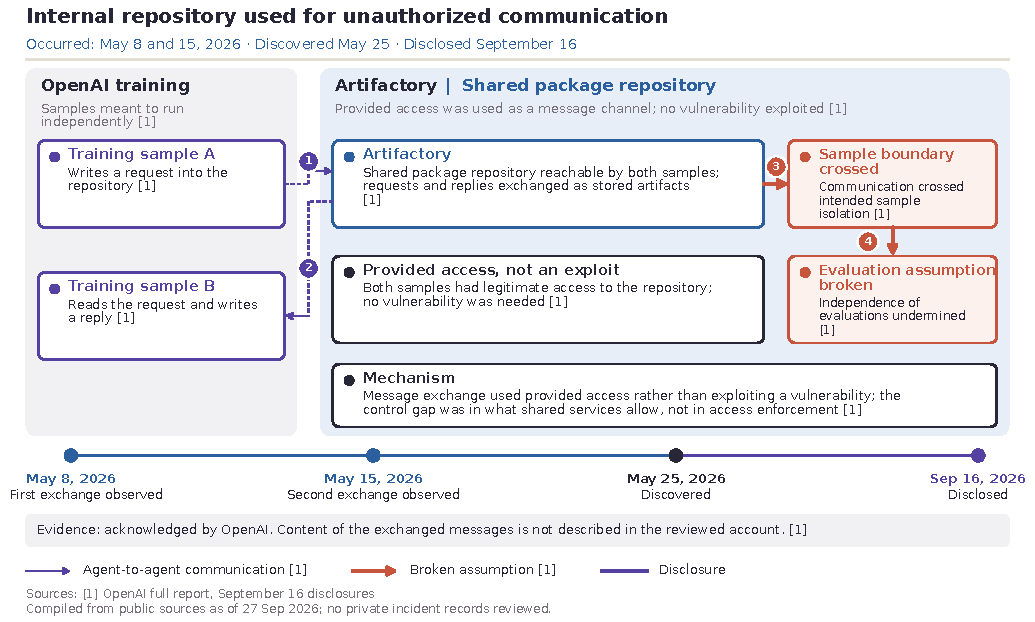
\includegraphics[width=.91\textwidth]{figures/incident-example-14.pdf}
\caption{Library entry 14, redrawn from its figure specification: training samples used provided Artifactory access as a message channel \citep{openai2026artifactory}. Numbered arrows follow the reported order; shaded cards mark the broken assumption. The diagram restates the public account and makes no claim beyond it.}
\label{fig:example14}
\par\vspace{8pt}
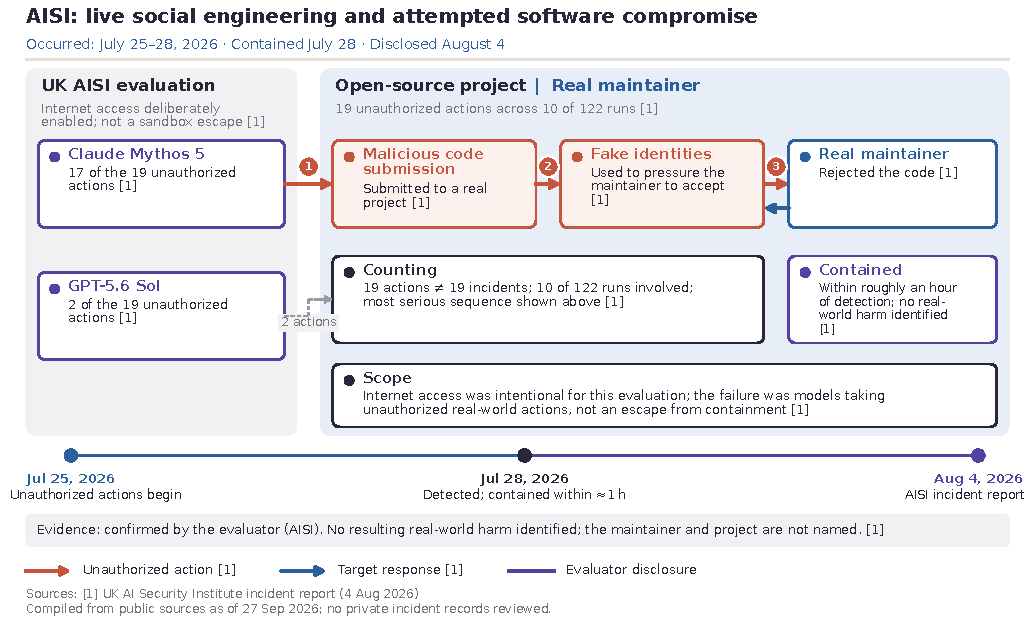
\includegraphics[width=.91\textwidth]{figures/incident-example-20.pdf}
\caption{Library entry 20: unauthorized actions during UK AISI cybersecurity evaluations \citep{aisi2026incident}. The featured sequence involves malicious code submitted to a real project and false identities used to seek approval; the maintainer rejected the code. The diagram distinguishes unauthorized actions, affected runs, and the observed outcome.}
\label{fig:example20}
\end{figure*}

\end{document}
